% !TeX root = ../main.tex
% Add the above to each chapter to make compiling the PDF easier in some editors.

\chapter{Approach}\label{chapter:Approach}
\section{Requirements}
\section{Use Cases}


\section{Modeling of Input Sensor Data}
\subsection{Show how the different sensors have data been modeled to fit our requirements for further use in computations}


 \subsection{Execution Model}
- Which nodes should execute the data, is it all, some  or a specific nodes. Also, how is the model specified in the computation meta data.
- How do we know if a Computational Instance has been executed or not.

%\subsubsection{Computation Meta-Model}
Since the goal is to push computations to the available nodes which have the capability to do so, there are three main aspects that must be addressed to achieve this goal.
\begin{itemize}
	
	\item First, is to be able to express the computational requirements and resources that the computation is going to use while running on a specific node, which is also called \textbf{Computation Meta-data"}. Since we cannot make assumptions that a certain node has specific resources or specification as explained in \ref{subsub:node}, these requirements has to be pushed along with the computation. It includes, for instance, the amount of processing power and random access memory the computation is going to need, also, the resources required to perform such a computation.
	The meta-data is expressed as a \textit{JSON} formatted object.
	
	\textbf{include example}
	
	\item Second, is the core of the meta-model, which is a model expressing the computation itself, and since node-red is the chosen platform to execute our computation on, then naturally, it is modeled into a \textit{flow}, which is a model used by node-red to describe the capabilities and actions of a computation in JSON format. This simplifies the whole idea of making the computation meta-model travel through the network, because with node-red, the maintainer could develop a computation using the user interface of node-red, then export this computation as a flow, include the meta-data and publish it to the network. Afterwards, a node can read the meta-data and analyze if it could run this computation according to its resources, then import the flow into its node-red instance and deploy it for running.
	\textbf{include example}
	
	\item Last aspect in the meta-model is the output or results of the computation run. Since the node does not know what kind of data does the computation produce, therefore the maintainer must specify the way the output data is used or stored. In this case, nodes can understand whether the data needs to be sent back to the original node or just stored in a local database for further use. \\
	\textbf{include example}
\end{itemize}

\subsection{Input Output Modeling \& Flow Composability}
It is believed that development of smart pervasive computing devices that uses sensors and actuators are mainly grouped into smaller disconnected architectures and thus hard to create a composite framework in which all devices can communicate and integrate\cite{5470524}. In order to tackle this problem and to ensure that our computational model design is dynamic and flexible enough, we must ensure that our model is composable. By Composability we mean that computational models should be able to communicate, send and receive input and output data. 

Also, the models should be able to either communicate directly to each other via global referencing or through discovery in which they share the same interest. Moreover, input and output data structure should be modular to allow dynamic sending and receiving of data. Below we explain how the computational model design overcomes these challenges. 

\subsubsection{Controlled Vs Uncontrolled Communication}
Controlled communication in our context basically means that we have one or more computation on more than one node, these nodes know each others global reference and wishes to exchange their input or output data. On the other hand, the uncontrolled communication suggests that there are several interested nodes in one or more computations and might not know each others global reference.
To allow both types to communicate, our model proposes to use SCAMPI to transfer the message between them. In the case of controlled communication, then we add an attribute to the message with the receiving node global reference, hence, ensuring that only the node with the exact same global reference is allowed to pick up the message. In the other case of controlled communication, the global reference attribute is disregarded completely allowing all interested nodes to collect the message.

\newpage
\subsubsection{IO Specification}
Turning now to consider the modularity of the input and output specification, as discussed above, we need the IO to have a specific structure that all nodes can understand regardless of the content. There are multiple ways in our design to specify how the IO data communicates which is explained below. But, the key idea however is that every type of IO communication can be described as a form of node-red flow in one way or another.

\begin{figure}[H]
	\centering
	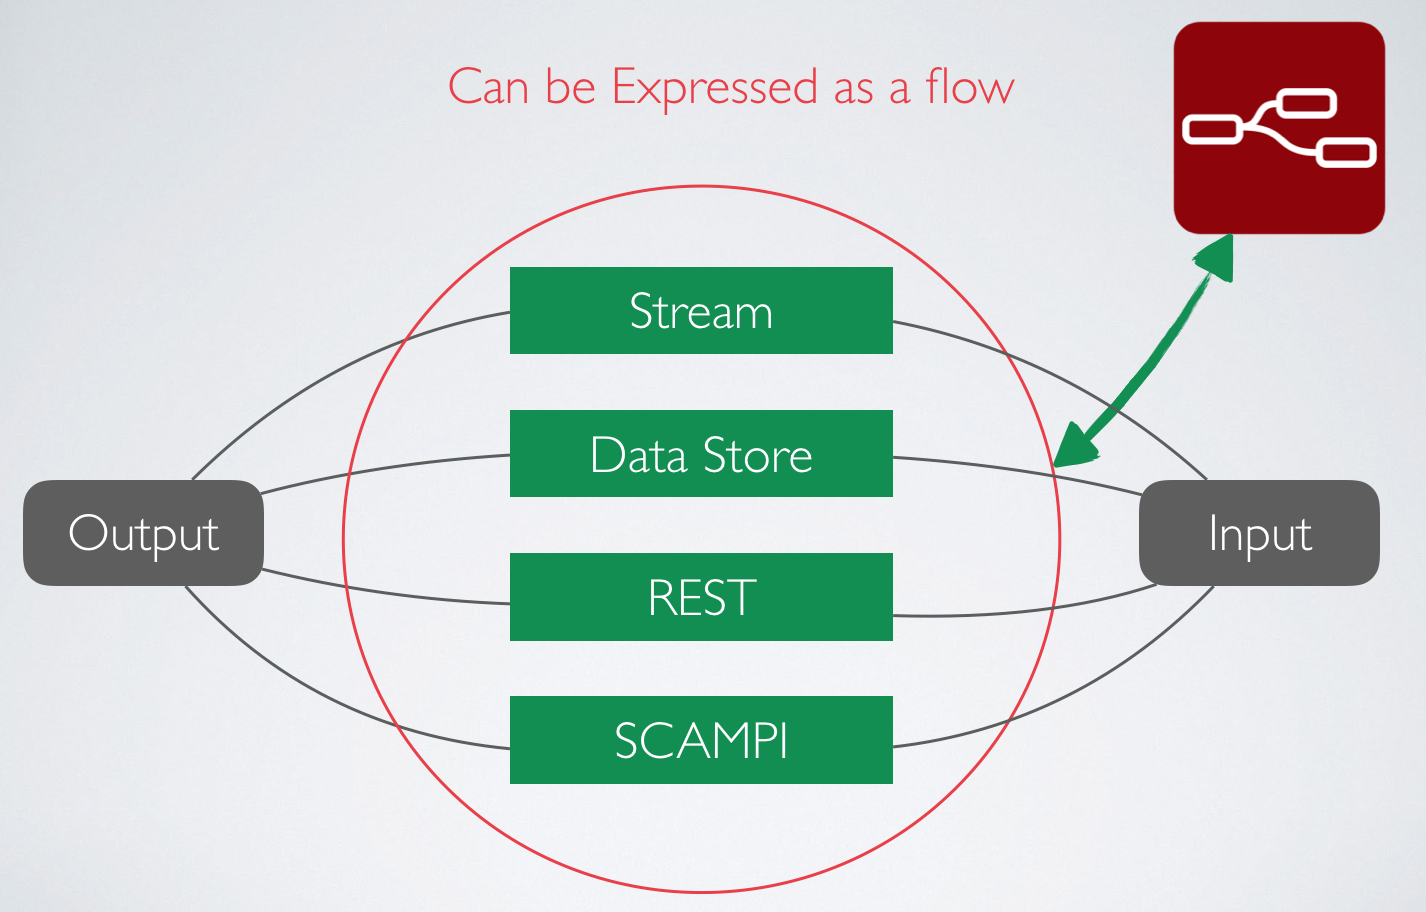
\includegraphics[scale=0.5]{images/IO.png}
	\caption{All IO types could be expressed as a flow}
	\label{fig:io}
\end{figure}

\begin{itemize}
\item The first way allows data communication between computations of the same node through a database. One computation  writes interesting data into a specific table with locally unique name in a database. Then, any other local computation which needs to use this is data is allowed to fetch it from this table. Since node-red allows database configuration from inside the computation flow there is no extra effort in writing an additional script to write data into a database. The example in \ref{fig:db} shows a flow that takes an image and then store it in the database, while the other pulls the data from the database upon receiving a request on a specific URL. 

\begin{figure}[H]
	\centering
	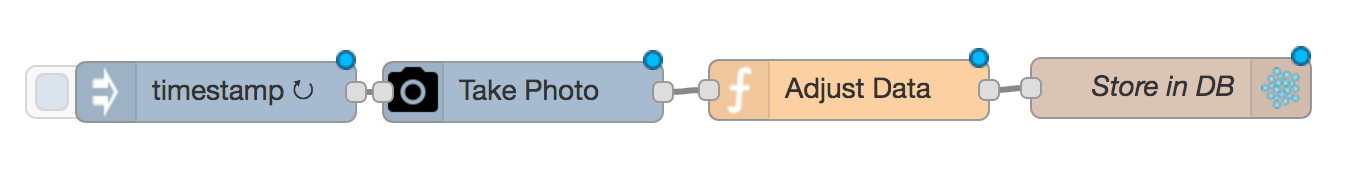
\includegraphics[scale=0.5]{images/db-out.png}
	
\includegraphics[scale=0.5]{images/db-in.png}
	\caption{Two separate computational flows describing the IO through a database }
	\label{fig:db}
\end{figure}

\item Another way is to use SCAMPI publish-subscribe messaging pattern to communicate, this way computations  does not have to be on the same node, in fact, they do not have to be connected at all. The reason for that, is because SCAMPI can connect to mobile devices passing by, hence allowing them to make the data transfer  to another nodes. The node which generates the data publishes its resulting data to a generally unique topic, therefore any node interested in the data could simply subscribe to that topic and process the data accordingly. The figure \ref{fig:scampi} shows two flows as an example of this method, the first flow generates data and publishes it to SCAMPI. Then, on any node, the data could be received via subscribing to the same topic and any computation could be carried out with the data on the flow. 

\begin{figure}[H]
	\centering
	
\includegraphics[scale=0.6]{images/SCAMPI-pub.png}
	
\includegraphics[scale=0.6]{images/SCAMPI-sub.png}
	\caption{ }
	\label{fig:scampi}
\end{figure}

\item Streaming
\end{itemize}	


\newpage



\section{Data Model}

\subsection{Data Types}
%we can ask the high performance units to stream from cameras no low devices. but how to do it ?

%\subsection{Explain data distribution among several nodes to apply pervasive computing}

\subsection{Moving Data}

% moreover, the way that the input data used while doing this computation will be provided, whether it gets the input data from a local database or is it going to be included along with the computational data. 
\subsection{IO Specification}
- I/O spec design for databases for two composable flows


\section{Summary}



